\documentclass[9pt,a4paper,twoside]{tau}
\usepackage[english, italian]{babel}
\usepackage{tauenvs}

%----------------------------------------------------------
% TITLE
%----------------------------------------------------------

\title{Lighting and Shading - Ray tracing}

%----------------------------------------------------------
% AUTHORS, AFFILIATIONS AND PROFESSOR
%----------------------------------------------------------

\author{Antonio Sirignano - Ciro Scognamiglio}

%----------------------------------------------------------

%\affil[a]{Affiliation of author one}
%\affil[b]{Affiliation of author two}
%\affil[c]{Affiliation of author three}

\professor{Calcolo Scientifico per l'Innovazione Tecnologica - prof. Luisa D'Amore}

%----------------------------------------------------------
% FOOTER INFORMATION
%----------------------------------------------------------

\institution{Università degli Studi di Napoli Federico II}
\ftitle{Lighting and Shading}
\date{a.a. 2023-2024}
\etal{Sirignano - Scognamiglio}
\course{Calcolo Scientifico per l'Innovazione Tecnologica}

%----------------------------------------------------------
% ABSTRACT
%----------------------------------------------------------

\begin{abstract}    
    In questo progetto viene fatta un'introduzione generale al lighting e allo shading, con una presentazione dei modelli di riflessione e di shading che possono essere applicati alla grafica computazionale. Viene poi presentato in maniera più approfondita il modello del ray tracing.
\end{abstract}

%----------------------------------------------------------

\keywords{calcolo scientifico, lighting, shading, ray tracing.}

%----------------------------------------------------------

\begin{document}
		
	\maketitle
	\thispagestyle{firststyle}
	\tauabstract
	\tableofcontents

%----------------------------------------------------------

\section{Introduzione}

    \taustart{L}a Computer Graphic Technology è l'abilità d produrre un effetto visivo realistico in un oggetto tridimensionale in un device di output bidimensionale, come un computer o un foglio stampato.\\
    Tutto ciò si ha grazie ai \textit{metodi di rendering} nei quali è applicato lo \textit{shading} per raggiungere il più possibile una rappresentazione di un oggetto vicina alla realtà.\\ 
    Infatti lo shading computa quantità e colore della luce emessa da ogni punto della superficie.\\
    Tali risultati dipendono dalle seguenti entità:
    \begin{enumerate}
    	\item \textbf{La sorgente di luce}. Intensità, colore, forma, direzione e distanza della sorgente di luce devono essere prese in considerazione e inoltre possono essere sia puntiformi che di grandi dimensioni.
    	\item \textbf{La superficie dell'oggetto}. L'oggetto può essere lucido, liscio, ruvido, brillante o scuro. Può inoltre avere colori differenti quali opachi, trasparenti o traslucidi. 
    	\item \textbf{L'ambiente}. Oggetti visti in uno spazio vuoto, senza un background che rifletta la luce su di essi, risultano duri (una navicella spaziale nello spazio profondo). Un modello realistico di shading deve tenere in considerazione la luce riflessa dagli altri oggetti (pareti vicine).
    \end{enumerate}

\section{Le sorgenti di luce}
\taustart{U}n oggetto illuminato dalla luce è colpito da raggi luminosi proiettati sulla sua superficie da un emittente chiamato \textit{sorgente di luce}. La luce può descrivere diverse scene presentate di seguito.
\begin{enumerate}
    	\item \textbf{Luce ambientale}. Questa luce è una sorgente di luce non direzione la cui luce è emessa da ogni direzione. La sua intensità è indipendente da tutte le sue caratteristiche, come posizione e orientamento.
    		\begin{figure}[H]
        		\centering
       			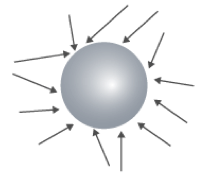
\includegraphics[width=0.3\columnwidth]{Figures/01.png}
       	 		\caption{Luce ambientale}
        		\label{fig:figure}
			\end{figure}
		
    	\item \textbf{Luce puntiforme}. \'E una sorgente di luce che non emette la stessa quantità di luce proveniente da tutte le direzioni, infatti un oggetto quanto è più vicino ad essa tanto è più luminoso. L'intensità della sorgente è quindi dipendente dalla distanza e dalla angolazione. \'E caratterizzata da colore, intensità, posizione e funzione di decadimento.
    		\begin{figure}[H]
        		\centering
        		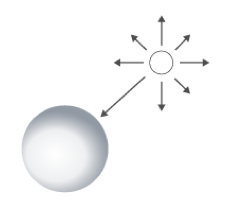
\includegraphics[width=0.3\columnwidth]{Figures/02.png}
        		\caption{Luce puntiforme}
       			\label{fig:figure}
			\end{figure}   
    	
    	\item \textbf{Luce direzionale}. Tale tipo è prodotta da una sorgente di luce da una distanza infinita dalla scena. Tutti i raggi di luce si espandano in una singola direzione e con la stessa intensità ovunque. \'E caratterizzata da colore, intensità e direzione.
    		\begin{figure}[H]
        		\centering
        		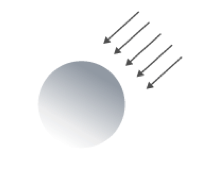
\includegraphics[width=0.3\columnwidth]{Figures/03.png}
        		\caption{Luce direzionale}
        		\label{fig:figure}
			\end{figure}
    	\item \textbf{Spotlight}. La luce si irradia in un cono con più luce al centro di esso. Questa luce è fissata all'asse primario di direzione con una restrizione su di essa. \'E caratterizzata come un punto di propagazione, un asse di direzione, un raggio intorno all'asse e la possibilità di una funzione di decadimento radiale. 
    		\begin{figure}[H]
		        \centering
		        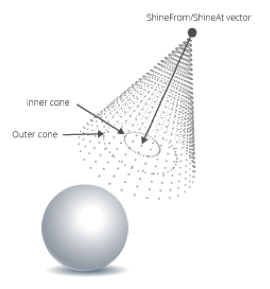
\includegraphics[width=0.3\columnwidth]{Figures/04.png}
		        \caption{Spotlight}
		        \label{fig:figure}
			\end{figure}
\end{enumerate}

\section{Modelli di riflessione}
L'obiettivo principale dello shading è la produzione di un risultato accettabile quando la superficie dell'oggetto è affetta dai raggi di luce. I modelli di riflessione sono presentati di seguito.
\begin{enumerate}
	\item \textbf{Riflessione diffusa} %TODO: riflessione diffusa
	\item \textbf{Riflessione speculare} %TODO: riflessione diffusa
\end{enumerate}

\section{Modelli di shading}
    
%\section{Document styling}
%
%    \subsection{Title}
%	
%        The \verb*|\maketitle| command generates the title and author information section, including the professor name or other information, and affiliations. The title can be modified in \textit{tau class} code in the \textit{title style} section. 
% 
%        By default, \textit{tau class} centers the title. However, you can change \verb*|\centering| to \verb*|\raggedright| in \verb*|\renewcommand{maketitle}| to move the title to the left or, modify it to your own preferences.
%	
%    \subsection{Abstract}
%	
%        The abstract and keywords are defined using the \verb*|\keywords| and \verb*|\begin{abstract} \end{abstract}| commands respectively. For the abstract to appear, make sure the \verb|\taucontent| command is always included after the beginning of the document.
%
%    \subsection{Table of contents}
%
%        The \textit{tau class} provides a table of contents. Each level of the ToC provides a preview of the content and its location in the document.
%
%    \subsection{Tau start}
%
%        We included the \verb*|\taustart{}| command, which provides a personalized lettrine for the beginning of a paragraph.
%        
%    \subsection{Caption}
%
%        \subsubsection{Figures}
%
%            The provided \verb*|\captionsetup[figure]| command customizes the appearance of captions for figures in \LaTeX\ documents. For example, in Fig. \ref{fig:figure}, shows an example figure.
%			
%            \begin{figure}[H]
%                \centering
%                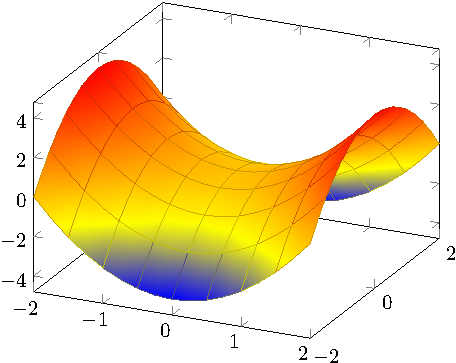
\includegraphics[width=0.8\columnwidth]{Figures/Example.pdf}
%                \caption{Example figure (obtained from \textit{PGFPlots - A LaTeX package to create plots}. [Online]. Available: \url{https://pgfplots.sourceforge.net/}).}
%                \label{fig:figure}
%            \end{figure}
%
%        \subsubsection{Tables}
%    
%            The \verb*|\captionsetup[table]| command customizes the appearance of the captions for tables in the document. The \verb*|\tabletext{}| is used to add notes to tables easily. Table \ref{tab:table}, shows an example table.
%            
%            \begin{table}[H]
%                \centering
%                \caption{Small table example.}
%    		\label{tab:table}
%                \begin{tabular}{cc}
%            	\toprule
%                    \textbf{Column 1} & \textbf{Column 2} \\
%                    \midrule
%                    Data 1 & Data 2 \\
%                    Data 3 & Data 4 \\
%                    \bottomrule
%                \end{tabular}
%                    
%                \tabletext{Note: I'm a table text for additional information.}
%                    
%            \end{table}
%
%    \subsection{Equation}
%    
%        Equation \ref{ec:equation} shows an example equation. 
%
%	\begin{equation} \label{ec:equation}
%            \frac{\hbar^2}{2m}\nabla^2\Psi + V(\mathbf{r})\Psi = -i\hbar \frac{\partial\Psi}{\partial t}
%	\end{equation} 
%
%        The \textbf{amssymb} package was not necessary to include, because the stix2 font incorporates mathematical symbols for writing quality equations. In case you choose another font, uncomment the package in \textit{tau class} code.
%
%        If you want to change the values that adjust the spacing above and below in the equations, go to \textit{tau class-math packages} section and play with \verb|\setlength{\eqskip}{6.5pt}| value until the preferred spacing is set. See appendix for more information.
%
%\section{Environment}
%
%    The \textit{tau class} includes custom environments designed to enhance the presentation of information within documents. Among these custom environments are \textbf{tauenv}, \textbf{info} and \textbf{note}.
%
%    \begin{tauenv}[frametitle=Custom title]
%        This is an example of the custom title environment. To add a title type \verb|[frametitle=Custom title]| next to the beginning of the environment (as shown in this example).
%    \end{tauenv}
%
%    One of the main features of the info and note environment is that they automatically change the language of their titles (currently English and Spanish).
%
%\section{Coding}
%
%    \textit{Tau class} includes the \textit{listings} package, which offers versatile and customizable features for typesetting code snippets in \LaTeX\ documents. Specifically for C, C++, \LaTeX\ and Matlab codes. 
%
%    For C and C++ codes, the \textit{listings} package recognizes the syntax of these programming languages and highlights keywords, comments, and string literals accordingly.
%
%    \lstinputlisting[caption=Example of C code., language=C]{example.c}
%
%    Similarly, for Matlab codes, the \textit{listings} package offers syntax highlighting and line numbering, to the MATLAB language syntax.
%    
%    \lstinputlisting[caption=Example of matlab code., language=Matlab]{example.m}
%
%\section{References}
%
%    The default formatting for references follows the IEEE style. This style is commonly used for technical documents, research papers, and scholarly articles in engineering fields \cite{einstein}.
%
%    At the end of the document, you will find an example of the default reference formatting \cite{dirac}.
%        
%\section{Appendix}
%
%    \subsection{Environments preview}
%
%        The following environments are defined in \textit{tauenvs} package.
%		
%		\subsubsection{Tau environment}
%
%                The following code defines the tauenv environment. A custom title can be added to this environment.
%
%			\begin{tauenv}[frametitle=Tauenv]
%                    Lorem ipsum dolor sit amet, consectetur adipiscing elit. Sed vestibulum justo quis massa aliquet, ut ultrices quam bibendum.
%			\end{tauenv}
%		
%\begin{lstlisting}[language=TeX, caption=Tauenv environment code.]
%\newmdenv[
%	backgroundcolor=taublue!22, 					
%	linecolor=taublue,									
%	linewidth=0.7pt,
%	frametitle=\vskip0pt\bfseries,
%	frametitlerule=false,
%	frametitlefont=\color{taublue}\bfseries\sffamily,
%	frametitlealignment=\raggedright,
%	innertopmargin=3pt,
%	innerbottommargin=6pt,
%	innerleftmargin=6pt,
%	innerrightmargin=6pt,
%	font=\selectfont,
%	fontcolor=taublue,									
%	frametitleaboveskip=8pt,
%	skipabove=10pt
%]{tauenv} \end{lstlisting}
%		
%		\subsubsection{Note}
%
%                This code defines the note environment.
%
%  			\begin{note}
%                    Lorem ipsum dolor sit amet, consectetur adipiscing elit. Sed vestibulum justo quis massa aliquet, ut ultrices quam bibendum.
%			\end{note}
%		
%\begin{lstlisting}[language=TeX, caption=Note environment code.]
%\newmdenv[
%	backgroundcolor=taublue!22, 						
%	linecolor=taublue,									
%	linewidth=0.7pt,
%	frametitle=\vskip0pt\bfseries\notelanguage,
%	frametitlerule=false,
%	frametitlefont=\color{taublue}\bfseries\sffamily,
%	frametitlealignment=\raggedright,
%	innertopmargin=3pt,
%	innerbottommargin=6pt,
%	innerleftmargin=6pt,
%	innerrightmargin=6pt,
%	font=\normalfont,
%	fontcolor=taublue,									
%	frametitleaboveskip=3pt,
%	skipabove=10pt
%]{note} \end{lstlisting}
%
%		\subsubsection{Info}
%
%                This code defines the info environment.
%
%    		\begin{info}
%                    Lorem ipsum dolor sit amet, consectetur adipiscing elit. Sed vestibulum justo quis massa aliquet, ut ultrices quam bibendum.
%			\end{info}
%		
%\begin{lstlisting}[language=TeX, caption=Info environment code.]
%\newmdenv[
%	backgroundcolor=taublue!22, 						
%	linecolor=taublue,									
%	linewidth=0.7pt,
%	frametitle=\vskip0pt\bfseries\infolanguage,
%	frametitlerule=false,
%	frametitlefont=\color{taublue}\bfseries\sffamily,
%	frametitlealignment=\raggedright,
%	innertopmargin=3pt,
%	innerbottommargin=6pt,
%	innerleftmargin=6pt,
%	innerrightmargin=6pt,
%	font=\normalfont,
%	fontcolor=taublue,									
%	frametitleaboveskip=3pt,
%	skipabove=10pt
%]{info} \end{lstlisting}
%
%    \subsection{Alternative title}
%
%         You can make the following modification to \textit{tau class} in the \textit{title preferences} section to change the position of the title. This will move the title to the left. 
%
%\begin{lstlisting}[language=TeX, caption=Alternative title.]
%\renewcommand{\@maketitle}{%
%        \vskip-18pt
%    {\RaggedRight\bfseries\color{taublue}\fontsize{18}{22}\sffamily\selectfont\@title\par}
%		\vskip8pt
%    {\RaggedRight\normalsize\sffamily\@author\par}
%        \vskip8pt
%    {\RaggedRight\fontsize{7pt}{8pt}\selectfont\@professor\par}
%        \vskip24pt
%}% 
%\end{lstlisting}
%
%    \subsection{Equation skip value}
%
%        Play with the value of \verb|\eqskip| until the preferred spacing is set for equations.
%
%\begin{lstlisting}[language=TeX, caption=Equation skip code.]
%\newlength{\eqskip}\setlength{\eqskip}{6.5pt}
%\expandafter\def\expandafter\normalsize\expandafter{%
%    \normalsize%
%    \setlength\abovedisplayskip{\eqskip}%
%    \setlength\belowdisplayskip{\eqskip}%
%    \setlength\abovedisplayshortskip{\eqskip-\baselineskip}%
%    \setlength\belowdisplayshortskip{\eqskip}%
%}
%\end{lstlisting}
					
%----------------------------------------------------------

\addcontentsline{toc}{section}{Riferimenti}
\nocite{*}
\printbibliography

%----------------------------------------------------------

%\begin{center}
%	\vskip10pt
%	Enjoy writing with tau \LaTeX\ class $\blacksmiley$ \\ 
%	\vskip10pt
%	\textit{Contact:} \\
%	\faLink\ \href{https://sites.google.com/view/memo-notess/p%C3%A1gina-principal}{https://sites.google.com/memo-notess} \\
%	\faEnvelope[regular]\ memo.notess1@gmail.com \\
%	\faInstagram\ memo.notess\\
%\end{center}

%----------------------------------------------------------

\end{document}